\documentclass{article}

\usepackage{graphicx}
\usepackage[utf8]{inputenc}

\title{Exabiome Journal}
\author{kellyhuang }
\date{August 2020}

\begin{document}

\maketitle

\section{Self-Attention Experiments}
Self-attention was used after the convolution layers and before the linear layers of Roznet. 

\subsubsection*{Small dataset: 200 epochs per run}
The following experiments were trained with these parameters: 
\newline
-M -g 4 -b 32 -s 3001 -S 1000 -W 1000 --lr 0.001

An accuracy of 96.72\% was achieved which is similar to the accuracy of Roznet without self-attention (96.38\%); however, this is because both accuracy scores are already very highly so the impact of self-attention isn't clearly demonstrated. 

\begin{figure}[h!]
  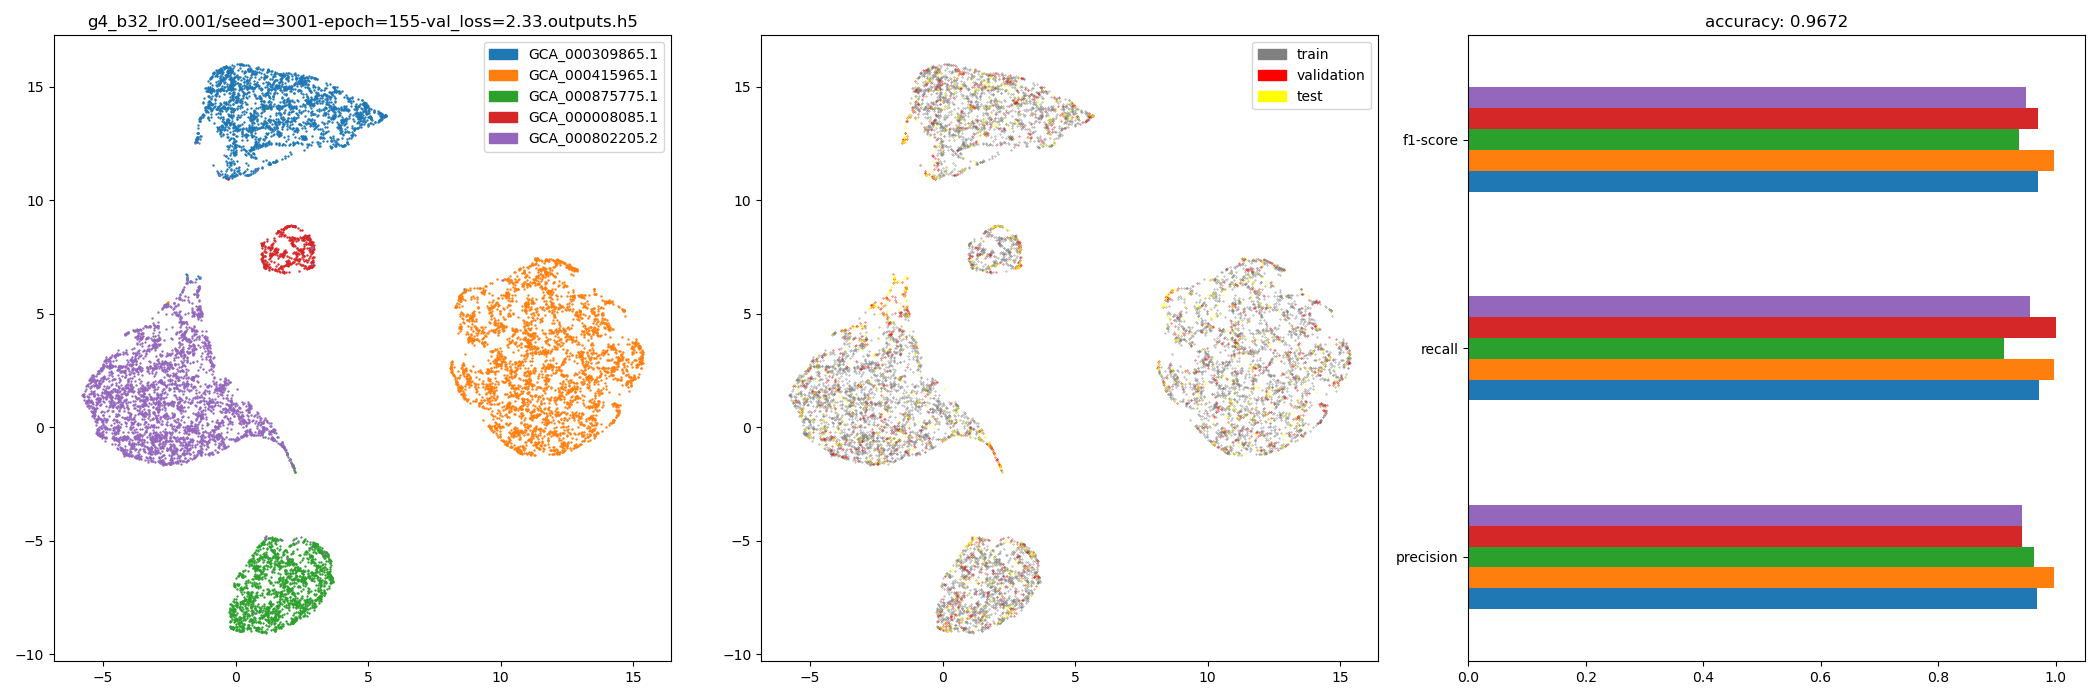
\includegraphics[width=\linewidth]{new_journal/figures/experiments/roznet_attn/small/e200.png}
  \caption{Run 1}
\end{figure}

\clearpage

\subsubsection*{Medium dataset - 88 epochs per run}
Each 4 hour run reached the maximum time limit at 88 epochs. The best results were achieved on the 187/264 epoch, with an accuracy of 77.43\% which is about 2\% higher than Roznet. After the third run, the validation loss began to fluctuate back up. Roznet with self-attention on the medium dataset seems to converge around an accuracy of 77\% after four 91 epoch runs.

\begin{figure}[h!]
  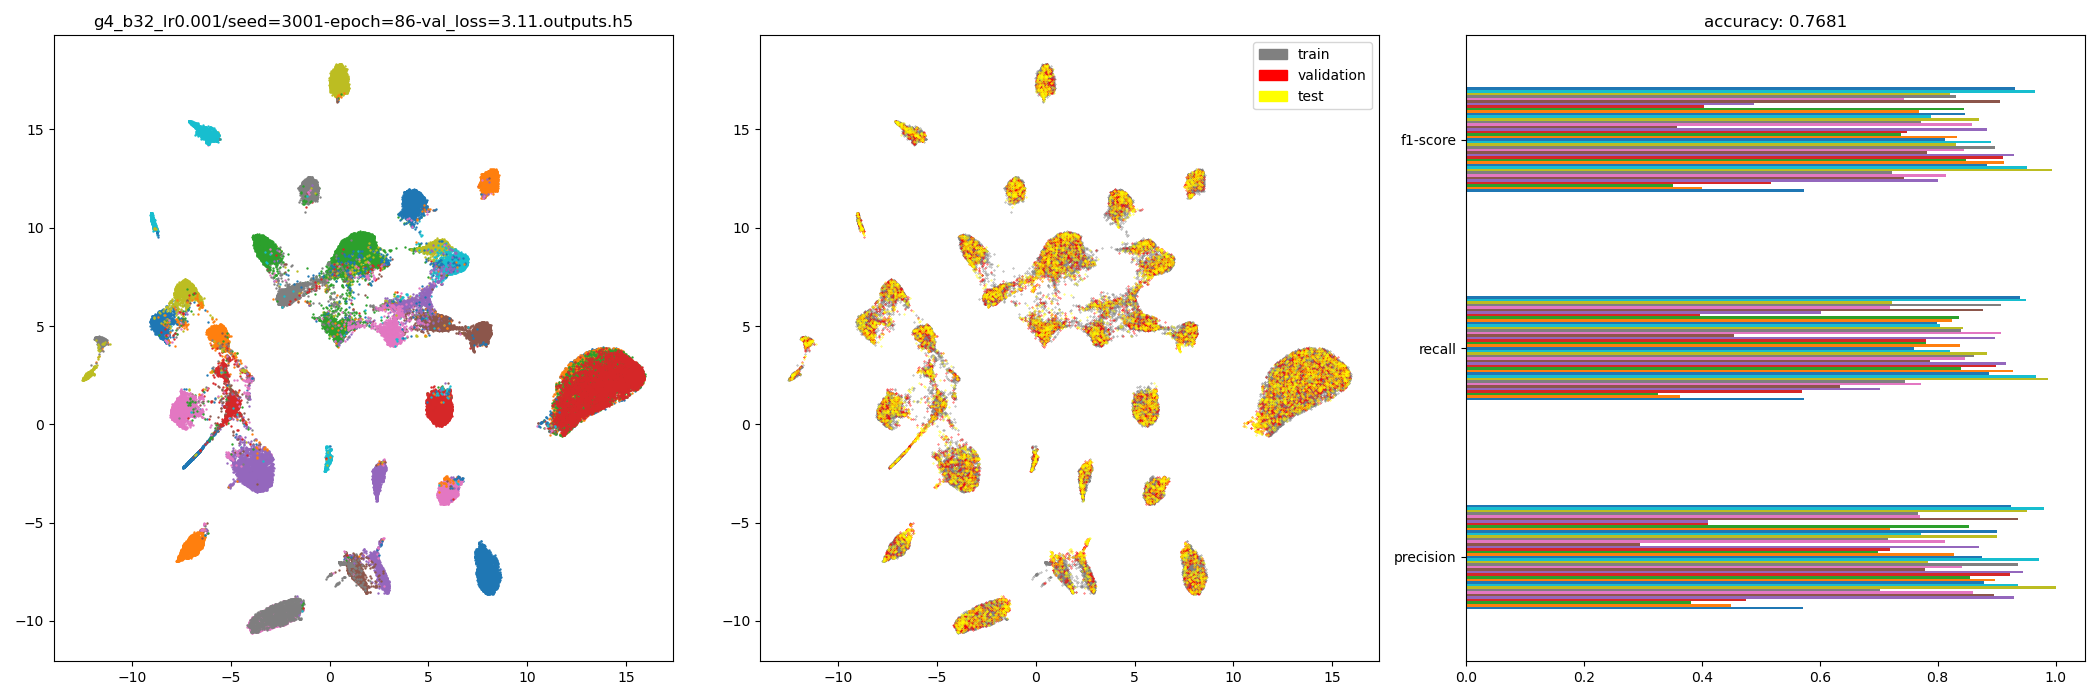
\includegraphics[width=\linewidth]{new_journal/figures/experiments/roznet_attn/medium/lr0.001/run1.png}
  \caption{Run 1}
\end{figure}

\begin{figure}[h!]
  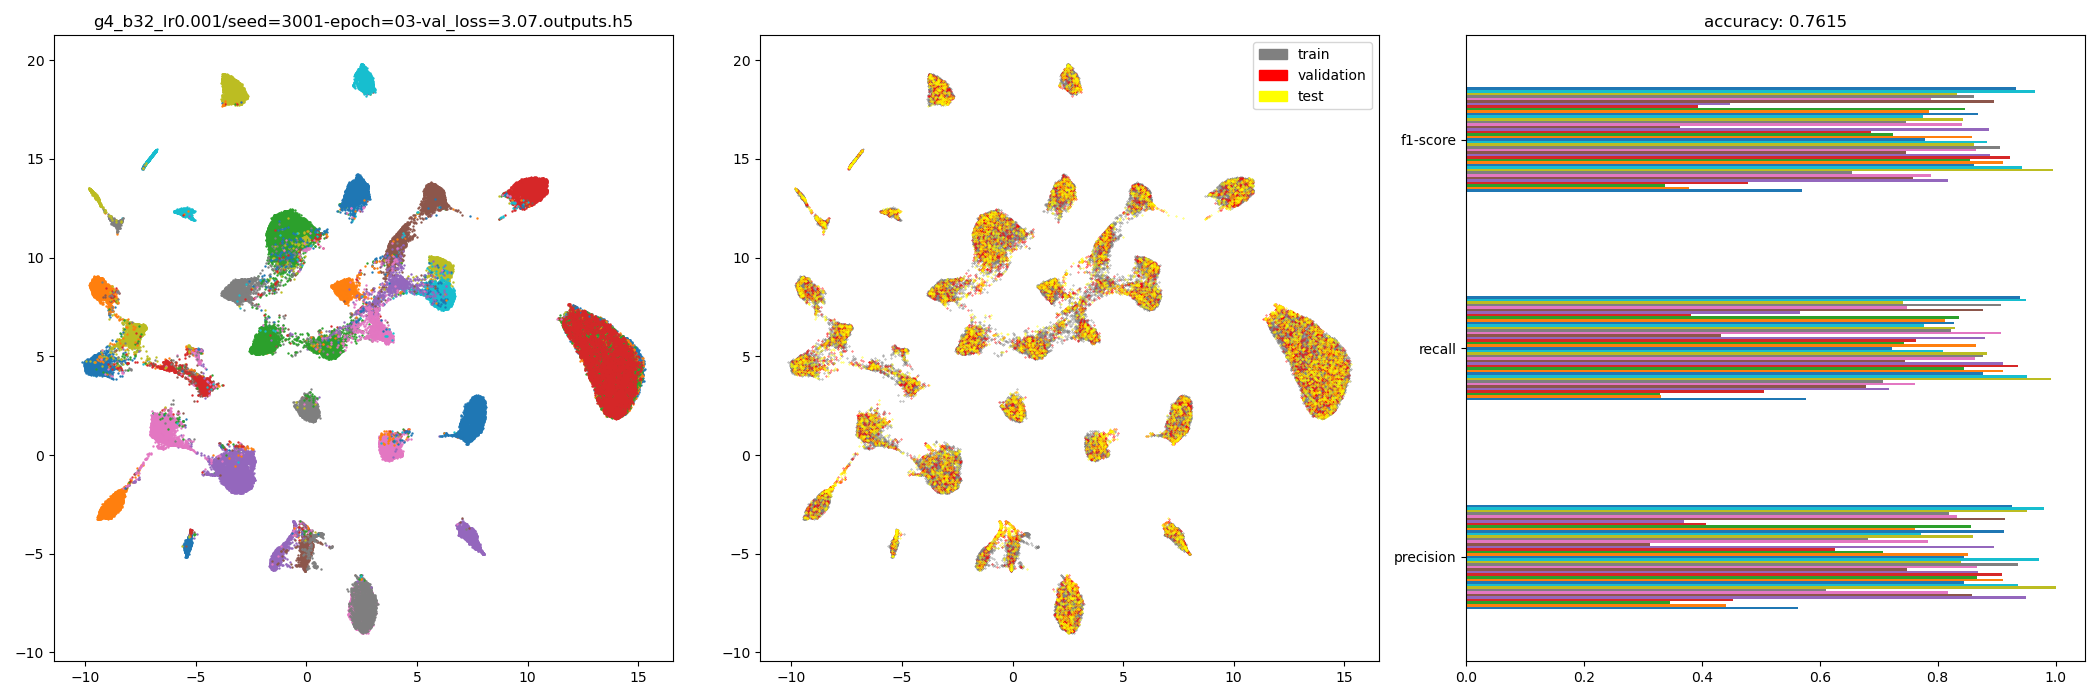
\includegraphics[width=\linewidth]{new_journal/figures/experiments/roznet_attn/medium/lr0.001/run2.png}
  \caption{Run 2}
\end{figure}

\begin{figure}[h!]
  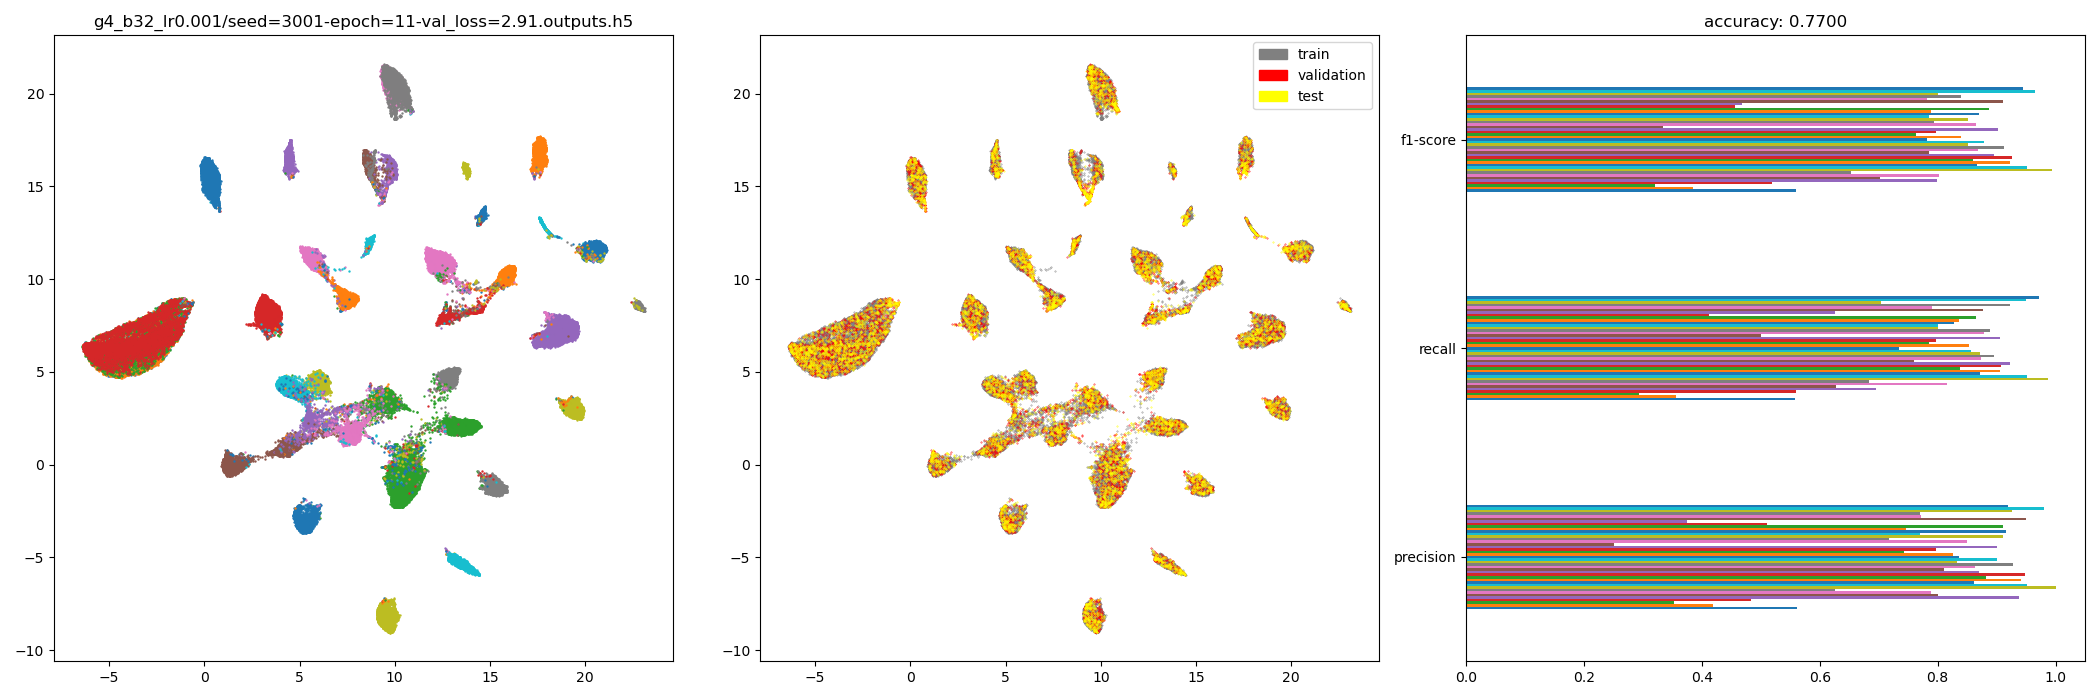
\includegraphics[width=\linewidth]{new_journal/figures/experiments/roznet_attn/medium/lr0.001/run3.png}
  \caption{Run 3}
\end{figure}

\begin{figure}[h!]
  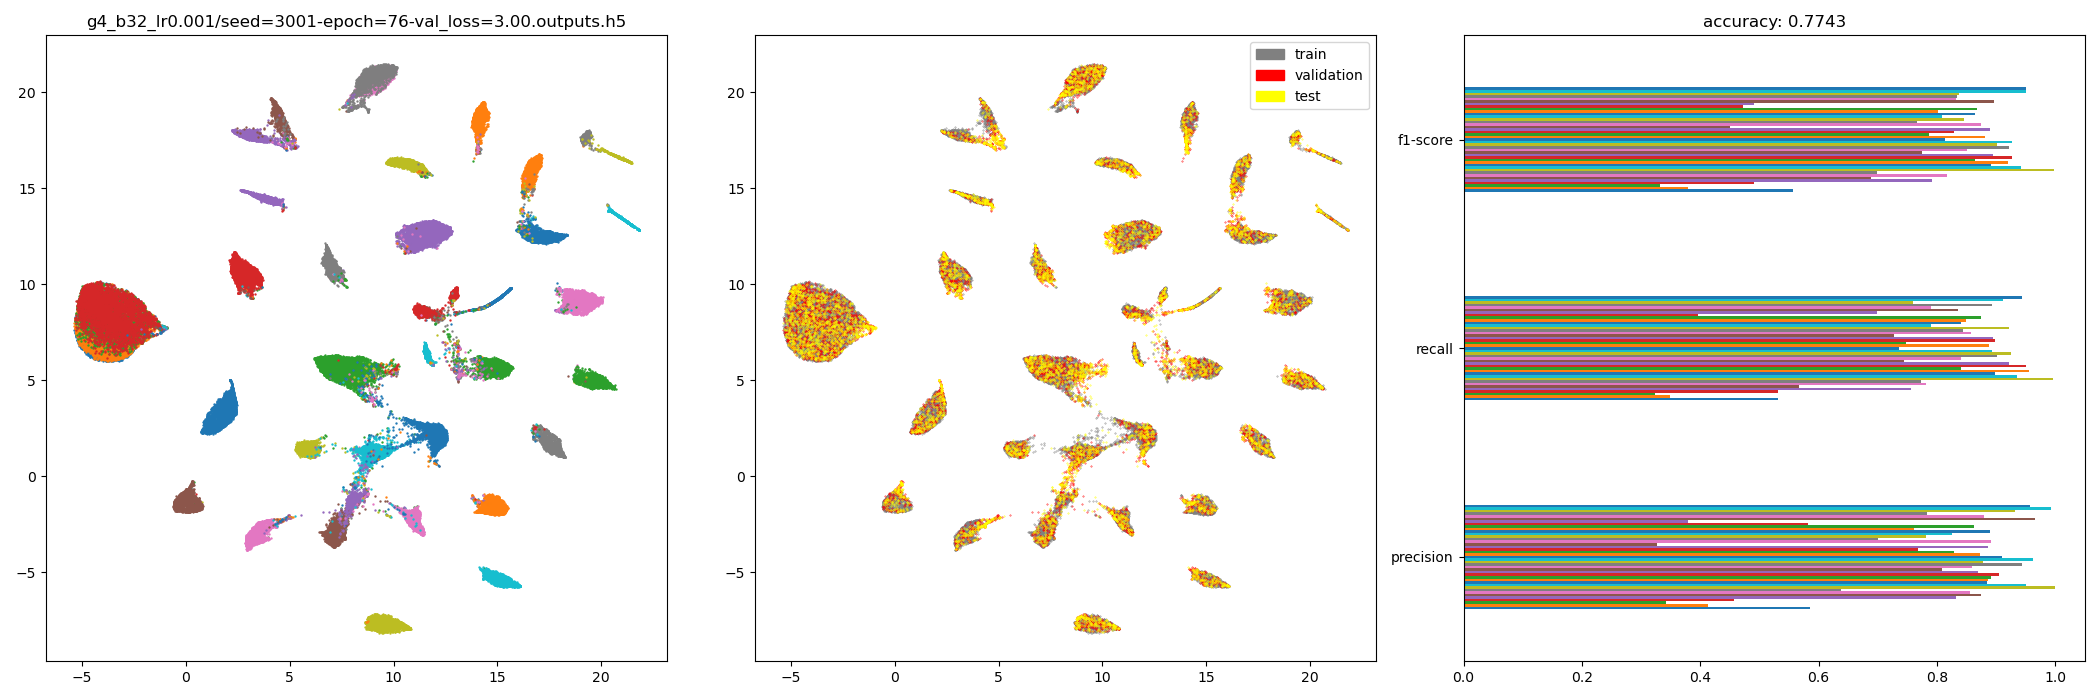
\includegraphics[width=\linewidth]{new_journal/figures/experiments/roznet_attn/medium/lr0.001/run4.png}
  \caption{Run 4}
\end{figure}

\clearpage

\subsubsection*{Medium dataset - 87 epochs per run}
The following experiments were trained with these parameters: 
\newline
-M -g 4 -b 32 -s 3001 -S 1000 -W 1000 --lr 0.0001

\begin{figure}[h!]
  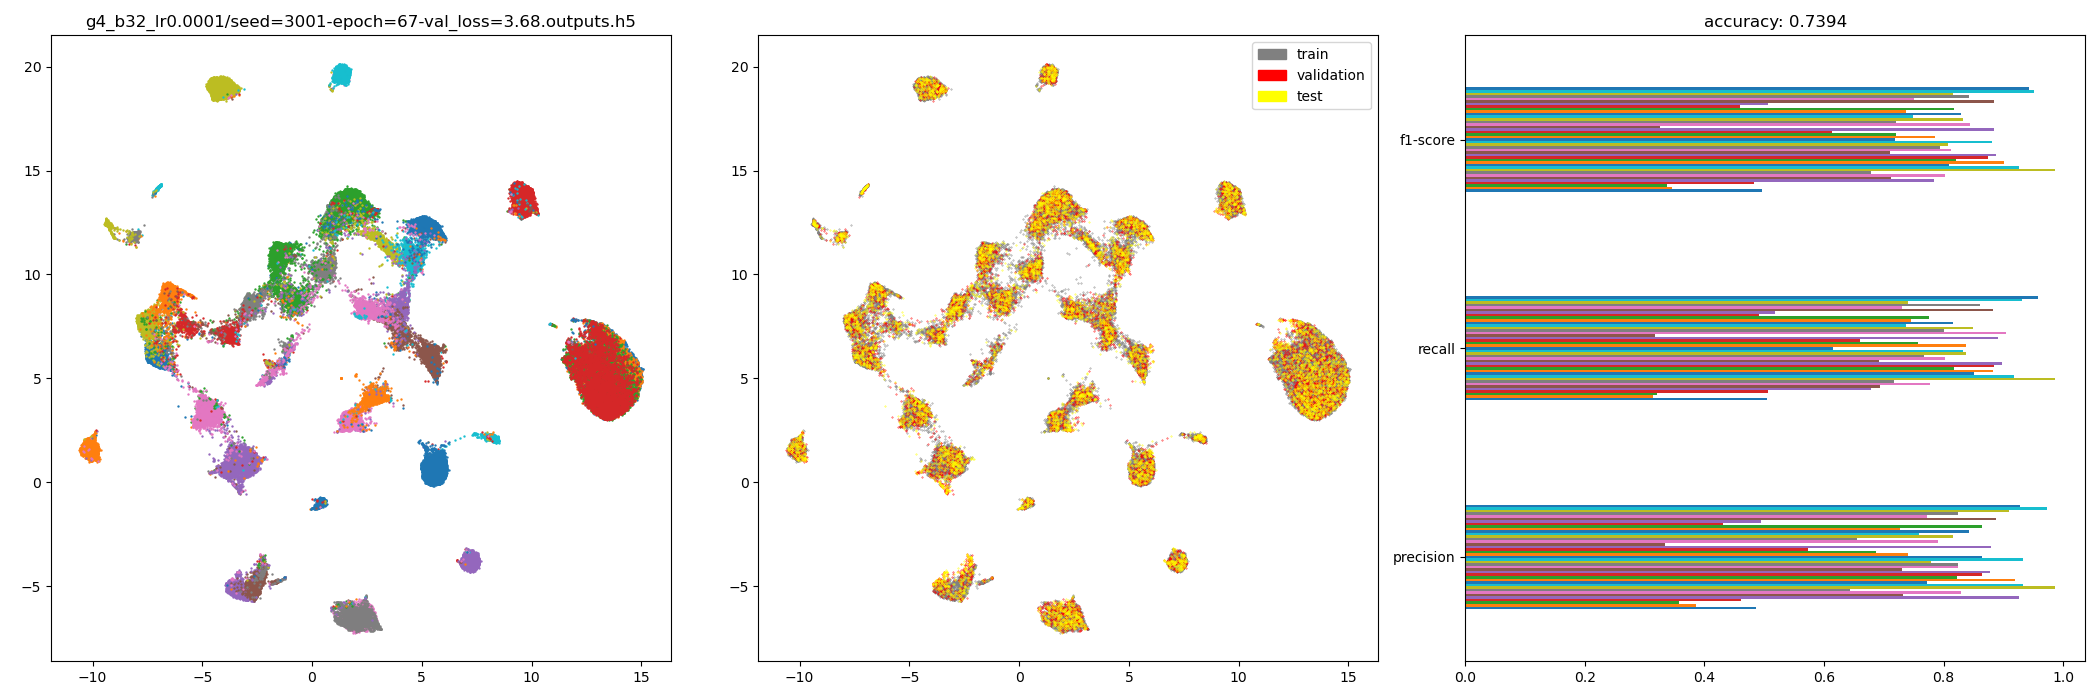
\includegraphics[width=\linewidth]{new_journal/figures/experiments/roznet_attn/medium/lr0.0001/run1.png}
  \caption{Run 1}
\end{figure}

\end{document}

